% LaTex-Dokument für Alexa Skill --------------------------
% Erstellt von Devin-A. Meier am 12.12.17 -----------------

%%%%%%%%%%%%%%%%% Begin des Dokuments %%%%%%%%%%%%%%%%%%%%%

\section*{Vorwort}
In dieser Arbeit wird die generelle Funktionsweise von Voice Assistants näher beleuchtet. Dazu wird zunächst geklärt, was unter einem Voice Assistant verstanden wird. Anschließend wird anhand eines vereinfachten Modells, der verallgemeinerte Ablauf eines Befehlaufrufs dargestellt. An dieser Stelle wird zudem auf die vereinzelten Bestandteile des genannten Modells näher eingegangen. Abschließend wird mithilfe von zwei Fallstudien der gesamte Ablauf konkret erläutert.
\newpage

\section{Was ist ein Voice Assistant?}
\label{secOne}
Voice Assistants (VAs) sind digitale Assistenten, welche Spracherkennung (SE),Computerlinguistik (CL) und Sprachsynthese (TTS) nutzen, um Nutzern auf Smartphones und Spracherkennungsgeräten verschiedene Dienste zur Verfügung zu stellen.

Um zu klären, was ein Voice Assistant ist, wird auf die obig genannten Begrifflichkeiten im folgenden näher eingegangen. Abschließend wird Anhand von historischen Beispielen die Entwicklung von Voice Assistants dargestellt.

\subsection{Digitaler Assistent}

Digitale Assistenten - auch Intelligente Persönliche Assistenten (IPA) genannt - sind Softwarelösungen mit der Fähigkeit der Spracherkennung und -analyse. Diese Fähigkeit erlaubt ihnen Anwender bei der Suche nach Informationen zu unterstützen und einfache Aufgaben für diese zu übernehmen. Ziel von digitalen Assistenten ist es Nutzern zu ermöglichen Suchanfragen und Kommandos einfacher zu formulieren. Hierzu sind IPAs in der Lage in einen Dialog mit dem Anwender zu treten. Dabei orientieren sich Fragen und Antworten immer mehr an einem normalen Gesprächsfluss.

\subsection{Spracherkennung}

Spracherkennung ist ein Teilgebiet der angewandten Informatik und Computerlinguistik. Das Ziel der Spracherkennung ist es Automaten die gesprochene Sprache zugänglich zu machen. Insbesondere helfen die entwickelten Verfahren Computern bei der automatischen Datenerfassung. Momentan wird zwischen zwei Arten der Spracherkennung unterschieden: Der sprecherunabhängigen und der sprecherabhängigen Spracherkennung. Während bei der sprecherunabhängigen Erkennung jeder Nutzer direkt erkannt wird, ist bei der sprecherabhängigen Erkennung ein kurzes Training des Systems nötig, um die Nutzererfahrung zu optimieren. Während erstere nur über einen Wortschatz von einigen Tausend Wörtern verfügen, erreichen letztere ein Vokabular von über 300.000 Worten.

\subsection{Computerlinguistik}

Computerlinguistik untersucht, wie natürliche Sprache von Computern algorithmisch Verarbeitet werden kann. Folgendes Zitat bietet eine gute Definition für den Begriff Computerlinguistik:

\begin{quotation}
	Computerlinguistik erforscht die maschinelle Verarbeitung natürlicher Sprachen. Sie erarbeitet die theoretischen Grundlagen der Darstellung, Erkennung und Erzeugung gesprochener und geschriebener Sprache durch Maschinen.
	
	- Universität München
\end{quotation}

Die Erfassung von Sprache ist Computern auf zwei Arten möglich. Sprache wird entweder als Schallinformation - akustisch - oder in Buchstabenketten - textuell - registriert.

Häufig wird bei der Verarbeitung das Saarbrücker Pipelinemodell genutzt, auf welches nun weiter eingegangen wird.

\newpage

\begin{enumerate}
	\item Spracherkennung \newline
	Umwandlung der Schallinformation in Text, falls nötig.
	\item Tokenisierung \newline
	Segmentierung der Buchstabenkette in Wörter und Sätze.
	\item Morphologische Analyse \newline
	Extraktion grammatischer Informationen und Rückführung der Wörter auf Grundform.
	\item Syntaktische Analyse \newline
	Analyse der einzelnen Wörter eines Satzes auf ihre strukturelle Funktion.
	\item Semantische Analyse \newline
	Zuordnung der Bedeutung einzelner Sätze. Kann viele Einzelschritte enthalten.
	\item Dialog- und Diskursanalyse \newline
	In Beziehung setzen aufeinander folgender Sätze.
\end{enumerate}

Zu beachten ist, dass durch maschinelles Lernen einige dieser Schritte ignoriert werden können. Dies lässt sich darauf zurückführen, das auf jeder Analyseebene statische Regelmäßigkeiten existieren, welche zur Modellierung zu Hilfe genommen werden können. Viele Modelle maschineller Übersetzung beschränken sich darauf Korrespondenzmuster auf Wortebene auszunutzen ohne Syntax und Semantik stark zu beachten. \newline


Momentan existieren drei Hauptprobleme bei der Sprachverarbeitung:
\begin{enumerate}
	\item Manche Sätze lassen sich auf mehrere Weisen deuten. Dementsprechend kann die Auflösung syntaktischer Mehrdeutigen zusätzliche semantische Informationen erfordern, allerdings mindestens ein statisches Vorwissen über gemeinsames Auftreten von Wörtern.
	\item Da die gleiche Wortform über unterschiedliche Bedeutungen verfügen kann - je nach Kontext -, gestaltet sich die Bestimmung der Semantik als schwierig.
	\item Einige Sätze sind nicht wörtlich gemeint. Die Absicht hinter dem gesagten muss erkannt werden, um eine korrekte Interpretation zu erhalten.
\end{enumerate}

\subsection{Sprachsynthese}
Sprachsynthese bezeichnet die künstliche Erzeugung der menschlichen Sprechstimme. Ein Text-to-Speech (TTS) System ermöglicht dies.

Bei der Erzeugung von Sprache unterscheidet man zwischen zwei verschiedenen Methoden. Einerseits kann durch den Zugriff auf Sprachaufnahmen eine Stimme modelliert werden. Diesen Vorgang bezeichnet man als Signalmodellierung. Andererseits kann die Stimme auch vollständig digital erzeugt werden. Dies wird als Formatsynthese bezeichnet.

Das größte Hindernis hierbei ist in beiden Fällen die Erzeugung einer Stimme mit natürlicher Sprachmelodie.

\subsection{Historie}

Den Grundstein für Voice Assistants legte Bell Laboratories 1952 mit dem ersten SE-Gerät namens AUDREY. AUDREY erkannte einzelne gesprochene Ziffern. Allerdings musste zwischen den gesprochenen Ziffern eine deutliche und klare Pause existieren. Da die Technologie noch nicht sehr ausgereift war und umständlich zu benutzen war, war sie kein kommerzieller Erfolg.

Im Jahr 1961 brachte IBM mit der IBM-Shoebox das erste kommerzielle SE-Gerät auf den Markt. Dieses erkannte 16 unterschiedliche Wörter, welche die Ziffern von 0-9 sowie die Befehle minus, plus, subtotal, total, false und of umfassten. Dadurch war das Gerät in der Lage einfache mathematische Operationen durchzuführen.

Die DARPA - Defense Advanced Research Projects Agency - entwickelte 1970 mit HARPY ein SE-Gerät welches bis zu 1000 Wörter erfassen konnte. 10 Jahre später erkannte HARPY durch Nutzung des Hidden Markov Models sogar ganze Sätze. Das Hidden Markov Model wird genutzt um die Wahrscheinlichkeit, dass ein bestimmtes Wort auf anderes folgt, zu bestimmen.

Der kommerzielle Durchbruch von VAs erfolgte am 4. Oktober 2011 mit der Veröffentlichung des iPhone 4S. Dieses verfügte über einen Voice Assistant namens Siri, welcher erstmals die Datenübertragung an einen Server zur Verarbeitung der Eingaben nutzte. Dadurch konnte der Funktionsumfang drastisch erhöht werden.

Heutzutage erfreuen sich eigenständige Voice Assistants immer größerer Beliebtheit. Nicht nur lassen sich diese Geräte überall im Haus aufstellen, sie verfügen auch über einen extrem erweiterbaren Funktionsumfang. Besonders bekannt sind die beiden Dienste Alexa des Unternehmens Amazon.com, Inc., welcher am 23. Juni 2015 erschienen ist, und Google Home des Unternehmens Alphabet Inc., welcher am 4. November 2016 herausgebracht wurde.
\newpage

\section{Generelle Funktionsweise eines Voice Assistant}
\label{secTwo}
In diesem Kapitel soll die generelle Funktionsweise eine Voice Assistants anhand eines Schaubilds dargestellt werden. Anschließend wird auf die einzelnen Bestandteile kurz eingegangen.

\begin{figure}[htb]
	\centering
	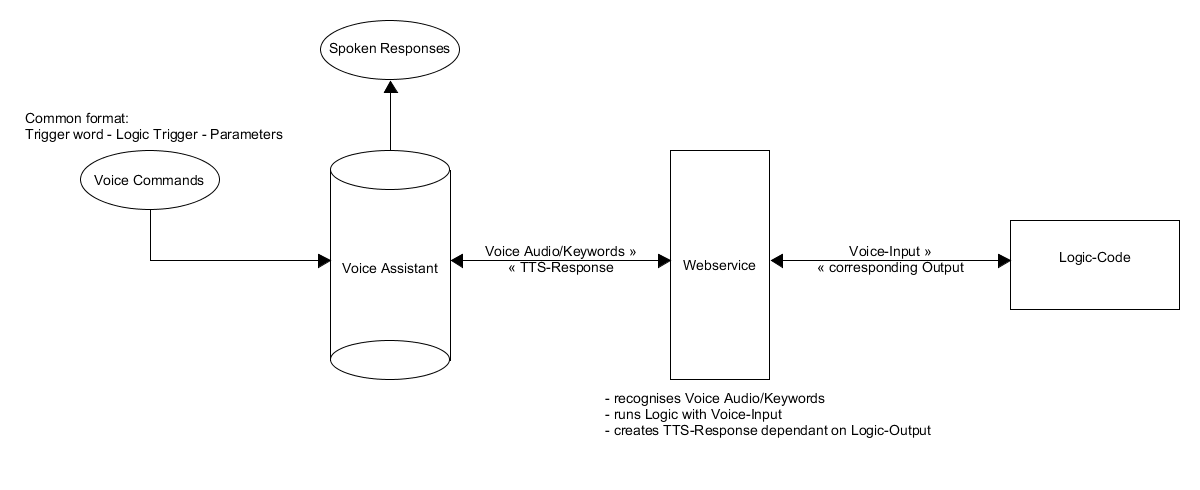
\includegraphics[scale=0.36]{content/img/GeneralVA_Architektur.png}
	\caption{Komponentendiagramm der generellen Funktionsweise eines Voice Assistants}
	\label{imgDiagramm}
\end{figure}

Wie in Abbildung \ref{imgDiagramm} beschrieben ist, muss der VA zunächst durch ein Trigger word aktiviert werden. Darauf folgt die so genannte Utterance. Diese setzt sich aus Logic Trigger und gegebenenfalls notwendigen Parametern zusammen. Diese wird mithilfe von SE auf dem Gerät erkannt und digitalisiert. Anschließend sendet der VA die Utterance an einen Webservice, der die weitere Verarbeitung übernimmt. So können die Voice Assistants schlank gehalten werden, da ein Großteil der Rechenarbeit auf dem Webservice erfolgt. \newline

Der Webservice erkennt nun anhand des Logic Triggers den konkreten Anwendungsfall und ermittelt, falls nötig, die gegebenen Parameter. Der konkrete Anwendungsfall wird als Intent bezeichnet. Die Anfrage wird daraufhin vom Webservice bearbeitet. Hierzu wird der auf einem Webserver abgelegten Logic-Code verwendet. Für jeden definierten Intent enthält der Logic-Code eine passende Funktion. Dies kann von einer einfachen Rechnung, über Suchanfragen im Internet bis hin zur Wiedergabe von akustischen Medien auf dem VA reichen.\newline

Der Logic-Code generiert eine zur Anfrage passenden Antwort, welche an den Webservice weitergereicht wird. Der Webservice erzeugt daraus eine TTS-Response, welche an den Voice Assistant gesendet wird. Letzterer ist nun in der Lage dem Anwender eine gesprochene Antwort auf seine Anfrage zu geben.

\subsection{Voice Assistant}
Im folgenden Schaubild wird veranschaulicht, was in Kapitel \ref{secOne} textuell beschrieben wird.
\begin{figure}[htb]
	\centering
	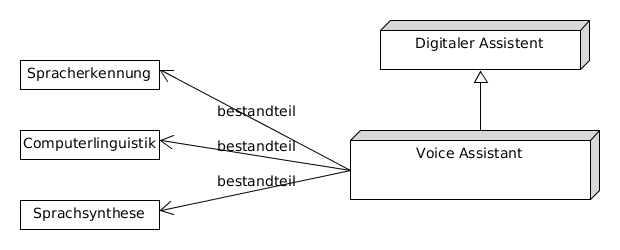
\includegraphics[scale=0.36]{content/img/bestandteile.png}
	\caption{Konzeptionelles Modell eines Voice Assistant}
	\label{imgBestandteile}
\end{figure}


\subsection{Webservice}

\subsection{Logic-Code}

\section{Alexa}
\label{secThree}

\section{Google Home}
\label{secFour}

%%%%%%%%%%%%%%%%%% Ende des Dokuments %%%%%%%%%%%%%%%%%%%%%
